\documentclass[a4paper]{scrartcl}
\usepackage[utf8]{inputenc}
\usepackage{ngerman}
\usepackage{mathtools}
\usepackage{amssymb}
\usepackage{pdfpages}
\usepackage{mathtools}
\usepackage{listings}
\usepackage{tikz}
\usepackage{qtree}
\usepackage{hyperref}
\usetikzlibrary{arrows,automata}
\usetikzlibrary{shapes.multipart}

\title{Künstliche Intelligenz}
\date{SS 2015}
\author{Markus Klemm.net}

\lstdefinestyle{customc}{
  belowcaptionskip=1\baselineskip,
  breaklines=true,
  frame=L,
  xleftmargin=\parindent,
  language=C,
  showstringspaces=false,
  basicstyle=\footnotesize\ttfamily,
  keywordstyle=\bfseries\color{green!40!black},
  commentstyle=\itshape\color{purple!40!black},
  identifierstyle=\color{blue},
  stringstyle=\color{orange},
}

\begin{document}
\maketitle
\tableofcontents

%Inhalte
%Prädikatenlogik
%Prolog-Programmierung
%Logisches Schließen
%Computeralgebra
%Sprachverarbeitung
%Problemlösen durch Suche
%%A*-Suche
%Bayes'sche Netze

\section{Prädikatenlogik}
\subsection{Problem} Aussagenlogik ist wenig mächtig. Aussagen, die sich nicht formulieren lassen:
\begin{itemize}
\item Alle Vögel können fliegen.
\item Wenn X eine Katze ist, dann ist X ein Haustier.
\item Für jedes Land gibt es eine Hauptstadt.
\end{itemize}
In der Prädikatenlogik betrachten wir zunächst eine (unwichtige) Menge $U$ (Universum), die alle zu betrachtenden Objekte (Vögel, Katzen, Länder) enthält.
Davon betrachten wir Teilmengen, z.B. die Menge aller Vögel (also eine einstellige Relation) oder die Menge aller Verheirateten (also eine mehrstellige Relation).
\subsection{Definition}
Sei $V$ eine Menge von Variablen, $K$ eine Menge von Konstanten, $F$ eine Menge von Funktionssymbolen.
\begin{itemize}
\item Dann sind alle Variablen in $V$ und Konstanten in $K$, Terme.
\item Wenn $t_1,\dots,t_n$ Terme und $f$ ein $n$-stelliges Funktionssymbol sind, dann ist auch $f(t_1,\dots,t_n)$ ein Term.
\end{itemize}
\paragraph{Beispiel} $V=\{x,y,z\},K=\{a,b,c\},F=\{+,*\}$ Terme sind $x,y,a,x+a,(x+a)*y$.

\subsection{Definition} Sei eine Menge von Prädikatensymbolen gegeben. Die Formeln der Prädikatenlogik sind induktiv.

\begin{itemize}
\item Wenn $t_1,\dots,t_n$ Terme und $P$ ein Prädikatensymbol der Stelligkeit $n$ ist, dann ist $P(t_1,\dots,t_n)$ eine Formel.
\item Wenn $F,G$ Formeln sind, dann auch $F \wedge G, F\vee G, \neg F$.
\item Wenn $x$ eine Variable und $F$ eine Formel sind, dann auch $\forall x F$, sowie $\exists x F$.
\end{itemize}
\paragraph{Beispiel} 
\begin{itemize}
\item katze(reni)
\item $\forall x (\text{katze}(x) \rightarrow \text{haustier}(x)) $
Syntaxbaum dazu \\* \begin{tikzpicture} 
\tikzstyle{level 1} = [sibling distance = 50 mm]
\tikzstyle{level 2} = [sibling distance = 30 mm]
\node{$\forall x$}
    child{node{$\rightarrow$}
        child{node{$\text{katze}(x)$}}
        child{node{$\text{haustier}(x)$}}
        }
        ;
\end{tikzpicture}
\item $\forall x(\text{land}(x) \rightarrow \exists y \text{hauptstadt}(x,y))$ \\*
\begin{tikzpicture} 
\tikzstyle{level 1} = [sibling distance = 50 mm]
\tikzstyle{level 2} = [sibling distance = 30 mm]
\node{$\forall x$}
    child{node{$\rightarrow$}
        child{node{$\text{land}(x)$}}
        child{node{$\exists y$}
            child{node{$\text{hauptstadt}(x,y)$}}
            }
        }
    ;
\end{tikzpicture}
\end{itemize}

\subsection{Semantik(informal)} Den Prädikatensymbolen müssen Relationen zugeordnet werden. Z.B: $\text{land} = \{\text{deutschland},\text{frankreich},\text{spanien}\}$\\
Wahrheitswert einer Formel:
\begin{itemize}
\item Die Formel $P(t_1,\dots,t_n)$ ist wahr, wenn $(t_1,\dots,t_n) \in P$
\item Die Wahrheit von $F \wedge G, F \vee G, \neg F$ ist wie in der Aussagenlogik definiert.
\item $\exists xF$ ist wahr, wenn es ein $x \in U$ gibt, so dass $F$ für dieses $x$ wahr ist.
\item $\forall xF$ ist wahr, wenn für alle $x \in U \quad F$ für diese $x$ wahr ist.
\end{itemize}
\paragraph{Beispiel}
\subparagraph{Symbole:} vogel,fliegt
\subparagraph{Relationen} $\text{vogel} = \{\text{amsel},\text{drossel},\text{fink},\text{star}\}, \text{fliegt} = \text{vogel} \cup \{\text{maikäfer},\text{A380}\}$
\begin{itemize}
\item $\text{vogel}(\text{amsel})$ ist wahr
\item $\exists x \; \text{vogel}(x)$ ist wahr
\item $\forall x \; \text{vogel}(x)$ ist falsch
\item $\forall x \; (\text{vogel}(x) \rightarrow \text{fliegt} (x))$ ist wahr
\end{itemize}

Vorrang der Operatoren:
\[ \begin{array}{c}
\neg \\
\forall \exists\\
\wedge, \vee\\
\rightarrow  , \leftrightarrow\\
\end{array}
\]

\paragraph{Beispiel} $\text{land} = \{\text{deutschland},\text{england},\text{frankreich},\text{spanien}\},$\\ $ \text{hauptstadt} = \{(\text{deutschland},\text{berlin}),(\text{england},\text{london}),(\text{frankreich},\text{paris}),(\text{spanien},\text{madrid}) \}$

\paragraph{Rechenregeln} 
\begin{itemize}
\item $\neg \forall x \; F \equiv \exists x \neg F$
\item $\neg \exists x \; F \equiv \forall x \neg F$
\item Für $Q \in \{ \forall, \exists \}$ und $\circ \in \{ \wedge, \vee \}$ gilt $(Q x F ) \circ G \equiv Q ( F \circ G )$, falls $x$ in $G$ nicht frei vorkommt.
\item $\forall x F \wedge \forall x G \equiv \forall x (F \wedge G)$
\item $\exists x F \vee \exists x G \equiv \exists x (F \vee G )$
\end{itemize}

\paragraph{Definition} Eine Aussage $F$ ist in bereinigter Pränexform wenn $F= Q_1 y_1 \dots Q_n y_n G$, wobei $Q_i \in \{ \forall , \exists \}$ und $G$ keine Quantoren enthält und $y_1,\dots,y_n$ paarweise verschieden sind.

Für jede Aussage gibt es eine äquivalente Formel in bereinigter Pränexform.

\subparagraph{Beispiel} \begin{align*} 
&\forall x ( \text{land} (x) \rightarrow \exists y \text{hauptstadt} (x,y)) &\equiv \\ 
&\forall x (\neg \text{land}(x) \vee \exists y \text{hauptstadt} (x,y)) &\equiv \\
&\forall x (\exists y \text{hauptstadt}(x,y) \vee \neg \text{land} (x)) &\equiv\\
&\forall x \exists y (\neq \text{land}(x) \vee \text{haupstadt}(x,y) ) &\equiv\\
&\forall x \exists y (\text{land} (x) \rightarrow \text{hauptstadt} (x,y))\\
\end{align*}

\begin{align*}
&\neg (\forall x(\text{vogel}(x) \rightarrow \text{fliegt} (x) ) ) &\equiv \\
&\neg (\forall x(\neg\text{vogel}(x) \vee \text{fliegt} (x) )) &\equiv \\
&\exists x \neg (\neg \text{vogel} (x) \vee \text{fliegt} (x) ) &\equiv \\
&\exists x (\text{vogel} (x) \wedge \neg \text{fliegt} (x))\\
\end{align*}

\paragraph{Definition}
\begin{itemize}
\item Ein \underline{Literal} ist eine Atomformel oder eine negierte Atomformel.
\item Eine Formel heißt \underline{Hornklausel}, wenn sie eine $\vee$-Verknüpfung von Literalen ist, von denen höchstens eins positiv ist.
\item Eine Hornformel ist eine $\wedge$-Verknüpfung von Hornklauseln.
\end{itemize}

\subparagraph{Beispiel}
\begin{itemize}
\item Literale: $P(x,y), \neg P(x,y), Q(zx)$\\
\item Hornklausel: $\neg P(x,y) \vee \neg Q(zx), \neg S(x) \vee T(y)$
\end{itemize}

\subparagraph{Wichtiger Spezialfall} Hornklausel mit genau einem positivem Literal.
\begin{itemize}
\item Ein Literal: Fakt, z.B. $P(x,y)$.
\item Mindestens zwei Literale: Dies lässt sich als Implikation darstellen.\\*
$ \neg A_1 \vee \dots \vee \neg A_{n-1} \vee A_n \equiv \neg (A_1 \wedge \dots \wedge A_{n-1} ) \vee A_n \equiv A_1 \wedge \dots \wedge A_{n-1} \rightarrow A_n$.
\end{itemize}

Mit Hilfe der Hornklausel lassen sich Regeln formulieren z.B.
\begin{align*}
&\forall x (\text{katze} (x) \rightarrow \text{haustier} (x)) &,\\
&\forall x (\text{hund} (x) \rightarrow \text{haustier} (x))&,\\
&\text{katze}(\text{reni})\\
\end{align*}
Wenn diese Hornklausel mit $\wedge$ verknüpft werden, erhalten wir eine Hornformel. Diese Hornformel kann als Wissensbasis eines Expertensystems betrachtet werden.

Grundlegender Aufbau eines Expertensystems
%TODO 2015-03-23T12:03 (Wissensbasis Inferenzsystem Anfrage Antwort

\section{Prolog-Programmierung}
\paragraph{Prolog} \underline{Pro}gramming in \underline{log}ic. In den 70ern und 80er Jahren als KI-Sprache entwickelt.

Prolog-Programme sind im Wesentlichen Hornformeln, bei denen alle Variablen allquantisiert sind und die in bereinigter Pränexform vorliegen.

Beispiel 
\begin{lstlisting}[numbers=left, tabsize=4, language=Prolog]
katze(reni).
haustier(X) :-katze(X).
\end{lstlisting}
Dieses Prolog-Programm stellt die Hornformel:
$\text{katze}(\text{reni}) \wedge \forall x(\text{katze}(x) \rightarrow \text{haustier}(x))$ dar.\\
Anfrage an Prolog:
\begin{lstlisting}[numbers=left, tabsize=4, language=Prolog]
? - haustier(reni).
true
\end{lstlisting}

\subsection{Syntax}
\paragraph{Prädikat} Wort in Kleinbuchstaben (außerhalb einer Klammer).
\paragraph{Konstante} Argument in Kleinbuchstaben.
\paragraph{Variablen} Wort, das mit Großbuchstaben beginnt.\\
"`$\leftarrow :$"' : "`$:-$"' (wird impliziert von)\\*
"`$\wedge$"' : "`,"'

Jede Klausel wird mit "`,"' abgeschlossen. Das Programm ist eine Menge von Klauseln, die implizit mit "`$\wedge$"' verknüpft sind (Hornformel).\\
$\vee$-Verknüpfung: Die Formel $A \vee B \rightarrow C$ ist wegen $A \vee B \rightarrow C \equiv \neq (A \vee B) \vee C \equiv (\neq A \wedge \neg B) \vee C$ keine Hornklausel. Da jedoch:
$A \vee B \rightarrow C \equiv (\neg A \vee C) \wedge (\neg B \vee C) \equiv (A \rightarrow C) \wedge (B \rightarrow C)$
eine Hornformel ist, lässt sich $A\vee B \rightarrow C$ in Prolog darstellen.

$\vee$-Operator: "`;"'\\*
Beispiel $\text{haustier}(X) :- \text{katze} (X); \text{hund}(x)$

\subsection{Unterschied zwischen Prolog und imperativen Programmiersprachen}
Eine Variable kann sowohl Ergebnis als auch Ausgabe sein.

\subparagraph{Beispiel}
\begin{lstlisting}[numbers=left, tabsize=4, language=Prolog]
katze(reni).
katze(mimi).
? - katze(reni).
true.
? - X=reni, katze(X).
true.
? - katze(X).
X=reni;
X=mimi.
\end{lstlisting}

\subsection{Behandlung von Existenzquantoren}
Da in Prolog alle Variablen allquantisiert sind, können existenzquantifizierte Variablen nicht unmittelbar dargestellt werden. Existenzquantoren können jedoch durch Skolemisierung. Dazu wird die Formel zuerst in bereinigte Pränexform gebracht.
\subparagraph{Einfacher Spezialfall} Die Formel in bereinigter Pränexform hat die Gestalt \[\exists x \; P(x)\]
Diese kann erfüllbarkeitsäquivalent dargestellt werden durch \[P(a)\] wobei $a$ eine noch nicht verwendete Konstante ist (Skolemkonstante).
\subparagraph{Weiterer Fall} Wenn die Formel die Gestalt
\[\forall x \exists y P(x,y)\]
besitzt, dann lässt sich diese erfüllbarkeitsäquivalent darstellen durch
\[P(x,f(x))\]
wobei $f$ ein noch nicht verwendetes Funktionssymbol ist (Skolemfunktion).

\subsection{Auswertestrategie von Prolog}
Die Struktur eines Prolog-Programms lässt sich durch einen Und-Oder-Baum darstellen.
\subsubsection{Und-Verknüpfung}
\begin{lstlisting}[numbers=left, tabsize=4, language=Prolog]
a(X) :- b(X),c(X),d(X).
\end{lstlisting}
[Bei folgendem Baum fehl noch ein Bogen um die Wurzel]\\*
\begin{tikzpicture} 
\tikzstyle{level 1} = [sibling distance = 50 mm]
\tikzstyle{level 2} = [sibling distance = 30 mm]
\node{$a(X)$}%TODO Kreis-Bogen um die Zweige (Zentrum root) als Und Konvetion
    child{node{$b(X)$}}
    child{node{$c(X)$}}
    child{node{$d(X)$}}
    ;
\end{tikzpicture}\\
Für die Anfrage $a(X)$ werden die Teilziele $b(X),c(X),d(X)$ erzeugt, die alle wahr sein müssen.
\subsubsection{Oder-Verknüpfung}
\begin{lstlisting}[numbers=left, tabsize=4, language=Prolog]
a(X) :- b(X);c(X);d(X).
\end{lstlisting}
\begin{tikzpicture} 
\tikzstyle{level 1} = [sibling distance = 50 mm]
\tikzstyle{level 2} = [sibling distance = 30 mm]
\node{$a(X)$}%ohne Kreisbogen
    child{node{$b(X)$}}
    child{node{$c(X)$}}
    child{node{$d(X)$}}
    ;
\end{tikzpicture}\\
Die Anfrage $a(X)$ ist wahr genau dann, wenn eines der Teilziele wahr ist $b(X),c(X),d(X)$ wahr ist.

\subsubsection{Suche nach einer Lösung} (d.h. $X$ ist nicht instanziert):\\
$X$ wird nach unten weitergereicht, bis es auf einer Blattebene an eine Konstante gebunden wird, mit der das zugehörige Teilziel war wird. Der so gefundene Lösungskandidat wird dann nach oben propagiert und für weitere Teilziele verwendet.\\
Bei folgendem Baum fehl noch ein Bogen um die Wurzel:\\*
\begin{tikzpicture} 
\tikzstyle{level 1} = [sibling distance = 50 mm]
\tikzstyle{level 2} = [sibling distance = 30 mm]
\node{$a(X)$}%TODO Kreis-Bogen um die Zweige (Zentrum root) als Und Konvetion
    child{node{$b(X)$}%TODO 2015-03-30T12:03
        child{node{$b(r)$}}
        }
    child{node{$c(X)$}}
    ;
\end{tikzpicture}\\
Wenn mit dem gefunden Kandidaten weitere, mit $\wedge$ verknüpfte Teilziele nicht erfüllbar werden, sucht Prolog nach weiteren Lösungen. Dazu wird eine Tiefensuche mit Backtracking ausgeführt.

\subparagraph{Beispiel} Aufgabe 4
Anfrage: $\text{nass}(\text{hochschulstraße})$\\
Bei folgendem Baum fehl noch ein Bogen um die Wurzel:\\*
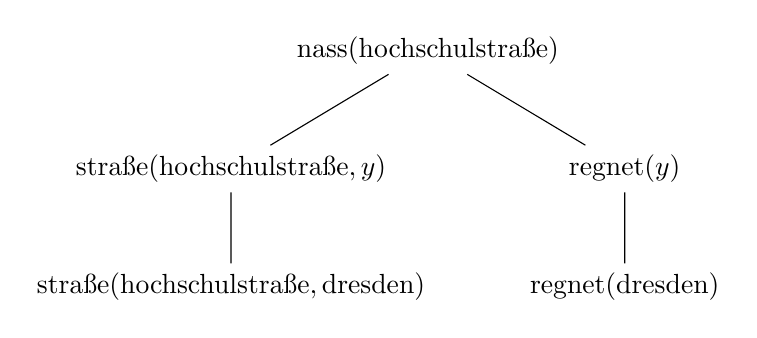
\begin{tikzpicture} 
\tikzstyle{level 1} = [sibling distance = 50 mm]
\tikzstyle{level 2} = [sibling distance = 30 mm]
\node{$\text{nass}(\text{hochschulstraße})$}%TODO Kreis-Bogen um die Zweige (Zentrum root) als Und Konvetion
    child{node{$\text{straße}(\text{hochschulstraße},y)$}%TODO 2015-03-30T12:03
        child{node{$\text{straße}(\text{hochschulstraße},\text{dresden})$}}
        }
    child{node{$\text{regnet}(y)$}
        child{node{$\text{regnet}(\text{dresden})$}}
        }
    ;
\end{tikzpicture}\\

\paragraph{Definition}
Zwei Atome $P,Q$ heißen \underline{unifizierbar}, wenn es eine Ersetzung der in $P,Q$ verkommenden Variablen gibt, so dass $P \equiv Q$.

\subparagraph{Beispiel} $\text{regnet}(y),\text{regnet}(\text{dresden})$ sind unifizierbar durch $y / \text{dresden}.$\\ $P(a,X,Y),P(a,b,c)$ sind unifizierbar durch $X/b,Y/c.$\\ $P(X,X),P(a,b)$ sind nicht unifizierbar.

\subsubsection{Durchsuchen des Baums} Für ein Ziel $P$ wird das Prolog-Programm von oben nach unten durchsucht, bis eine linke Seite einer Klausel(Kopf) mit $P$ unifiziert. Dadurch wird ein neues Ziel erzeugt. Wenn dieses neue Ziel false liefert, wird ein Backtracking ausgeführt, indem eine weitere linke Seite gesucht wird, die mit dem Ziel unifiziert. Innerhalb jeder Klausel wird die rechte Seite von links nach rechts durchsucht.
\paragraph{Problem bei der Tiefensuche}
Beispiel: 
\begin{lstlisting}[numbers=left, tabsize=4, language=Prolog]
zug(X,Y) :- zug(Y,X).
zug(1,2).
?- zug(2,1).
\end{lstlisting}
Suchbaum\\
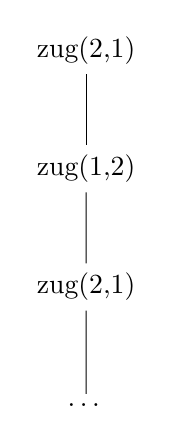
\begin{tikzpicture} 
\tikzstyle{level 1} = [sibling distance = 50 mm]
\tikzstyle{level 2} = [sibling distance = 30 mm]
\node{zug(2,1)}
        child{node{zug(1,2)}
            child{node{zug(2,1)}
                child{node{\dots}}
            }
        }
    ;
\end{tikzpicture}\\
Da der Suchbaum unendlich ist, liefert die Tiefensuche keine Lösung.

Lösung: Klauseln anders anordnen: Abbruchbedingung der Rekursion nach oben:
\begin{lstlisting}[numbers=left, tabsize=4, language=Prolog]
zug(1,2).
zug(X,Y) :- zug(Y,X)
\end{lstlisting}











\end{document}